\documentclass[UTF8,zihao=-4]{ctexart}

\usepackage[a4paper,margin=2.4cm]{geometry}
\usepackage{array}
\usepackage{booktabs}
\usepackage{longtable}
\usepackage{tabularx}
\usepackage{enumitem}
\usepackage{xcolor}
\usepackage{graphicx}
\graphicspath{{figure/}{output/pdf/figure/}}
\usepackage{hyperref}
\usepackage{fancyhdr}
\usepackage{titlesec}
\usepackage{float}

\definecolor{Primary}{HTML}{155B64}
\definecolor{Accent}{HTML}{8A5A2B}
\definecolor{Soft}{HTML}{F4F7F6}
\definecolor{Good}{HTML}{2E7D32}
\definecolor{Risk}{HTML}{B26A00}

\hypersetup{
  unicode=true,
  colorlinks=true,
  linkcolor=Primary,
  urlcolor=Accent,
  pdftitle={信息学竞赛 AI 自动造数据与数据校验工具需求报告},
  pdfauthor={专业实习项目组}
}

\pagestyle{fancy}
\setlength{\headheight}{15pt}
\fancyhf{}
\cfoot{\thepage}

\titleformat{\section}{\Large\bfseries\color{Primary}}{\thesection}{0.8em}{}
\titleformat{\subsection}{\large\bfseries\color{Accent}}{\thesubsection}{0.8em}{}
\setlist[itemize]{leftmargin=2em,itemsep=0.2em,topsep=0.3em}
\setlist[enumerate]{leftmargin=2em,itemsep=0.2em,topsep=0.3em}
\renewcommand{\arraystretch}{1.3}
\setlength{\parskip}{0.45em}
\setlength{\parindent}{2em}
\emergencystretch=2em

\newcommand{\projectname}{信息学竞赛 AI 自动造数据与数据校验工具}
\newcommand{\statusok}{\textcolor{Good}{建议纳入 应用}}
\newcommand{\statuslater}{\textcolor{Risk}{需二次确认}}
\newcommand{\statusno}{\textcolor{Risk}{暂不纳入 应用}}

\begin{document}

\begin{titlepage}
  \centering
  \vspace*{2cm}
  {\Huge\bfseries \projectname \par}
  \vspace{0.8cm}
  {\LARGE 需求方业务逻辑与界面确认报告\par}
  \vspace{1.2cm}
  {\large 面向需求方二次确认\par}
  \vfill
  \begin{tabular}{rl}
    报告用途： & 确认业务流程、功能范围与界面方案 \\
    项目阶段： & 专业实习项目设计阶段 \\
    编制日期： & 2026 年 7 月 9 日 \\
  \end{tabular}
  \vfill
\end{titlepage}

\tableofcontents
\newpage

\section{业务逻辑总览}

\subsection{业务流程图}

\begin{center}
\fbox{\begin{minipage}{0.92\textwidth}
\centering
创建项目 \\
$\downarrow$ \\
填写题目描述、C++ 标程和难度等级（均为必填；难度仅归档） \\
$\downarrow$ \\
编译检查标程 \\
$\downarrow$ \\
AI 生成、用户修改并确认输入结构 \\
$\downarrow$ \\
按子任务配置数据范围、测试点数量、期望复杂度和特殊测试点 \\
$\downarrow$ \\
生成并确认 generator 和 validator 草稿，支持多次换种子试运行 \\
$\downarrow$ \\
安全环境中批量生成输入数据 \\
$\downarrow$ \\
校验输入数据并运行标程生成标准输出 \\
$\downarrow$ \\
导出代码与配对的输入输出数据
\end{minipage}}
\end{center}

\subsection{每一步的业务含义}

\begin{longtable}{p{3.2cm}p{6.2cm}p{4.4cm}}
\toprule
步骤 & 用户感知 & 系统处理 \\
\midrule
阶段 1：创建项目 & 填写题目描述、C++ 标程和难度等级 & 保存项目；三项均为必填，难度等级仅用于归档，不作为 AI 输入 \\
阶段 2：标程编译检查 & 查看编译结果与日志 & 在 Docker 环境编译标程；失败时保留已有输入供用户修改 \\
阶段 3：输入结构确认 & 在多行文本框中审核、编辑并确认 AI 生成的输入结构 Template 与完整问题清单 & 综合题目和标程读取逻辑，以一致变量名按读取顺序生成非结构化输入描述；确认后保存为 Template，AI 与用户未共同确认或仍有阻碍问题时继续迭代 \\
阶段 4：子任务规划 & 左栏查看只读 Template，右栏通过可扩展表单配置各子任务 & 每个子任务以自由文本配置数据限制，并配置数量、复杂度和非规模性特殊测试点；如需修改 Template 返回阶段 3，AI 核验与用户确认后继续 \\
阶段 5：代码草稿与试运行 & 预览 generator、validator，并可多次更换种子运行 & 生成并检查代码及试运行结果；AI 核验与用户确认后继续，否则迭代 \\
阶段 6：批量生成 & 等待生成结果 & 在 Docker 环境编译并按已确认配置批量生成 \texttt{.in} 文件；资源受限或生成失败时提示重试、调整或终止；合法数据数量不足时补充生成，按原因返回阶段 4 或 5 \\
阶段 7：校验与输出 & 查看合法数据、失败原因和 \texttt{.out} 生成结果 & 使用 validator 校验输入，并运行标程生成配对输出；校验失败或标程运行异常时展示原因，规划问题返回阶段 4，生成器或校验器问题返回阶段 5 \\
阶段 8：导出 & 下载 zip 数据包 & 导出 \texttt{generator.cpp}、\texttt{validator.cpp} 和最终 \texttt{.in/.out} 文件 \\
\bottomrule
\end{longtable}

\subsection{确认与迭代规则}

AI 完成任一任务后，不能直接决定反馈或通过。系统需将任务要求、相关上下文和执行结果交由 AI 再次检查，并由该检查返回确认字段；只有确认字段表示通过，流程才可继续。未通过时，系统根据检查结果报错或重新执行、检查和迭代。

阶段 3、阶段 4 和阶段 5 除需通过上述 AI 检查外，还必须由用户明确确认；任一条件未满足时，不得进入下一阶段。

\subsection{输入、子任务配置与文件规则}

\begin{longtable}{p{3.2cm}p{4.1cm}p{6.2cm}}
\toprule
配置项 & 输入方式 & 规则 \\
\midrule
题目描述 & 多行文本框或文本文件上传 & 必填；支持粘贴或上传 Markdown 等文本文件，填写题意、输入格式、输出格式和必要说明。 \\
C++ 标程代码 & 代码编辑器或 \texttt{.cpp} 文件上传 & 必填；支持粘贴或上传，保存后需通过编译检查。 \\
难度等级 & 单选下拉框 & 必填；由用户选择题目难度，仅用于归档，不作为 AI 输入。 \\
输入结构 Template & AI 生成的可编辑多行文本框 & 阶段 3 综合题目描述和标程读取逻辑，以一致变量名按实际读取顺序生成完整的非结构化输入描述；用户可审核修改，确认后自动保存为 Template。 \\
子任务数据限制 & 可编辑自由文本框 & 阶段 4 左栏只读展示 Template，右栏每个子任务提供数据限制文本框。支持自然语言、数学不等式、变量与范围的键值形式、区间形式和分行文本，不要求统一句式；含义明确的轻微名称差异由 AI 规范，只有无法可靠解析、真正歧义或冲突才报告问题。 \\
子任务测试点数量 & 数值输入框 & 必填；为正整数，包含普通测试点和本子任务的全部特殊测试点。 \\
期望通过的算法复杂度 & 单选下拉框 + 条件文本框 & 必填；提供常见复杂度和“其它”。选择“其它”时，具体复杂度文本框必填。 \\
非规模性特殊测试点 & 可扩展子表单 & 每项仅填写测试点数量和描述；子表单数量之和不得超过所属子任务的总测试点数量；不需要时可为空。 \\
种子试运行 & 种子输入与运行操作 & 阶段 5 可按子任务指定种子，也可多次更换种子运行生成器并预览结果。 \\
输入输出文件命名 & 系统默认生成 & 以“子任务号\_内部编号”配对命名；两个编号均为无前置零的自然数，扩展名固定为 \texttt{.in} 和 \texttt{.out}，例如 \texttt{1\_1.in/1\_1.out}、\texttt{1\_2.in/1\_2.out}、\texttt{2\_1.in/2\_1.out}。 \\
\bottomrule
\end{longtable}

\section{功能范围确认}

\subsection{建议纳入 应用 的功能}

\begin{longtable}{p{4cm}p{9.5cm}}
\toprule
功能 & 说明 \\
\midrule
单题项目管理 & 创建、查看、编辑单题项目  \\
标程导入与编译 & 上传 C++ 标程并检查是否能编译  \\
题目描述配置 & 支持通过多行文本框录入，或上传 Markdown 等文本文件  \\
难度等级配置 & 通过单选下拉框选择难度等级，仅用于归档，不作为 AI 输入  \\
输入结构确认 & AI 基于题目描述和标程读取逻辑，在可编辑文本框中生成采用一致变量名的非结构化输入描述及完整问题清单；共同确认后保存为 Template，否则持续迭代  \\
可扩展子任务规划 & 页面左栏只读展示输入 Template，右栏每行代表一个可增删子任务；每个子任务包含自由文本数据限制、测试点数量、期望复杂度和非规模性特殊测试点  \\
子任务数据限制文本 & 用户可用自然语言、不等式、键值范围、区间或分行文本描述范围与关系，无需重复输入结构或改写为固定句式；轻微名称差异由 AI 规范，无法可靠解析、真正歧义、冲突或 Template 错误时才反馈  \\
特殊测试点子表单 & 每项只包含测试点数量和描述；特殊测试点与普通测试点合计为该子任务总数，特殊项数量之和不得超出总数；不需要时可为空  \\
AI 自检与共同确认 & AI 每次执行后根据任务要求、上下文和结果进行二次检查并返回确认字段；未通过时报告问题或重新执行；阶段 3 至 5 还需用户明确确认  \\
生成器与校验器草稿 & 生成并展示 \texttt{generator.cpp} 与 \texttt{validator.cpp}，根据反馈反复修改  \\
种子试运行 & 支持用户传入或更换种子，多次运行生成器预览数据后再确认批量生成  \\
批量输入生成 & 在 Docker 环境中编译并批量生成 \texttt{.in} 文件  \\
输入校验与标准输出生成 & 使用 validator 保留合法输入，并使用用户标程生成对应 \texttt{.out}  \\
zip 导出 & 仅导出 \texttt{generator.cpp}、\texttt{validator.cpp} 及最终 \texttt{.in/.out}；以“子任务号\_内部编号”配对命名，两个编号均为无前置零的自然数  \\
\bottomrule
\end{longtable}

\subsection{暂不纳入应用需要二次确认的功能}

\begin{longtable}{p{4cm}p{9.5cm}}
\toprule
功能或事项 & 暂不纳入原因或需确认问题  \\
\midrule
OJ 平台兼容 & 无法理解需求方的"兼容OJ平台,课堂练习,模拟比赛”是什么具体需求,需要兼容什么。 \\
SPJ 自动生成 & 特殊评测通常需要完整题面和输出判定规则，仅通过标程代码难以可靠推断。  \\
交互题 & 交互题的执行、输入输出协议和校验机制与普通题不同，需要单独设计。  \\
\bottomrule
\end{longtable}

\clearpage
\section{界面设计展示}

下列图片用于展示当前原型的页面布局与操作路径。其中如存在与前述八阶段流程不一致的字段、流程或“报告导出”等历史表述，均不作为需求确认依据；实施时必须以本报告的业务逻辑、功能范围和导出规则为准。

\begin{figure}[H]
  \centering
  \colorbox{white}{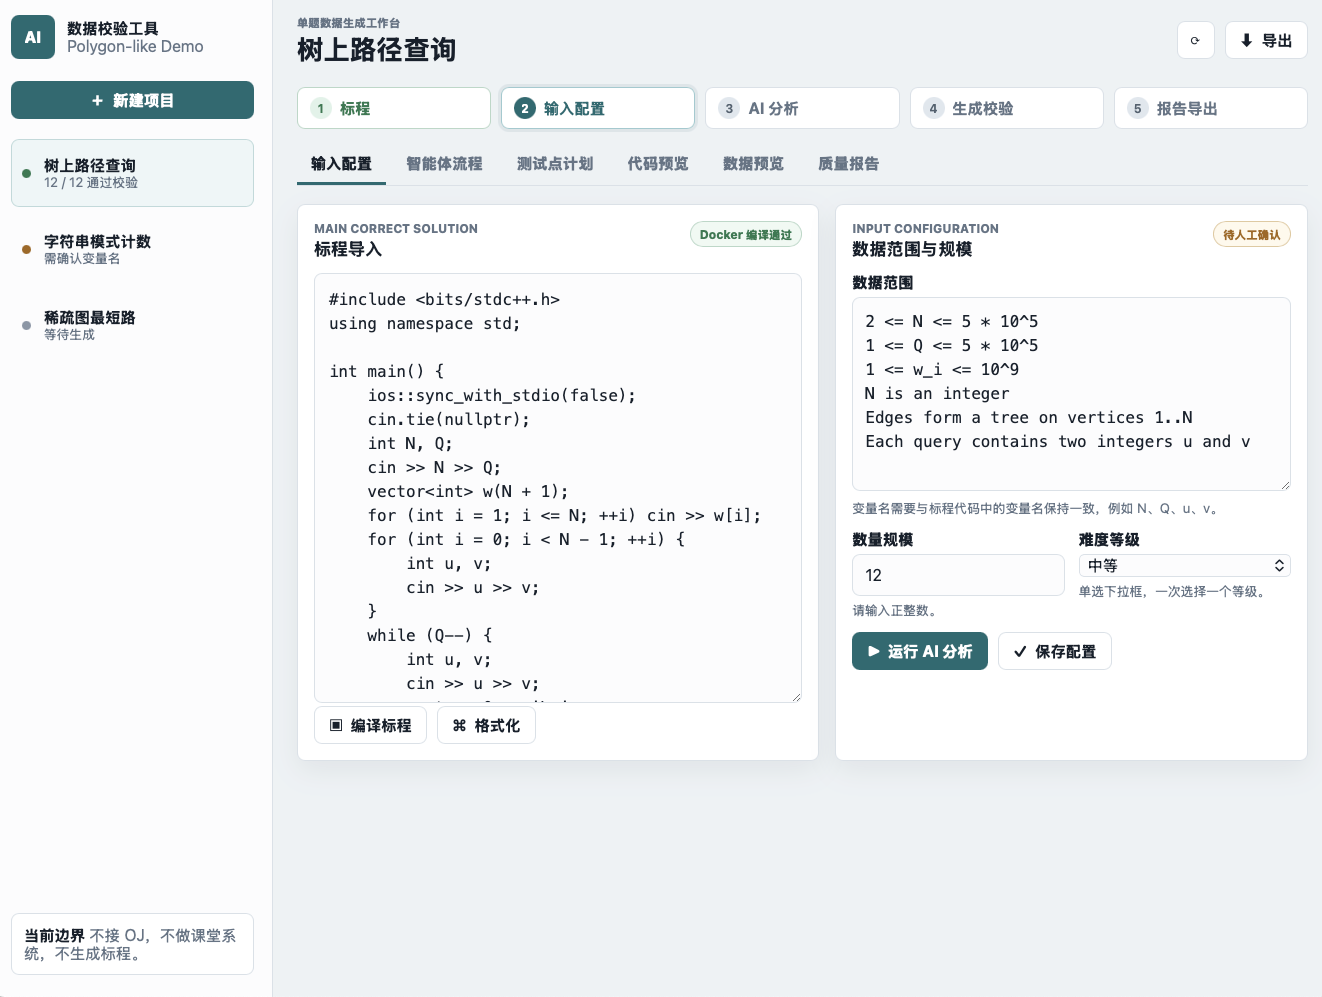
\includegraphics[width=0.8\textwidth]{输入配置.png}}
  \caption{输入配置原型}
\end{figure}

\begin{figure}[H]
  \centering
  \colorbox{white}{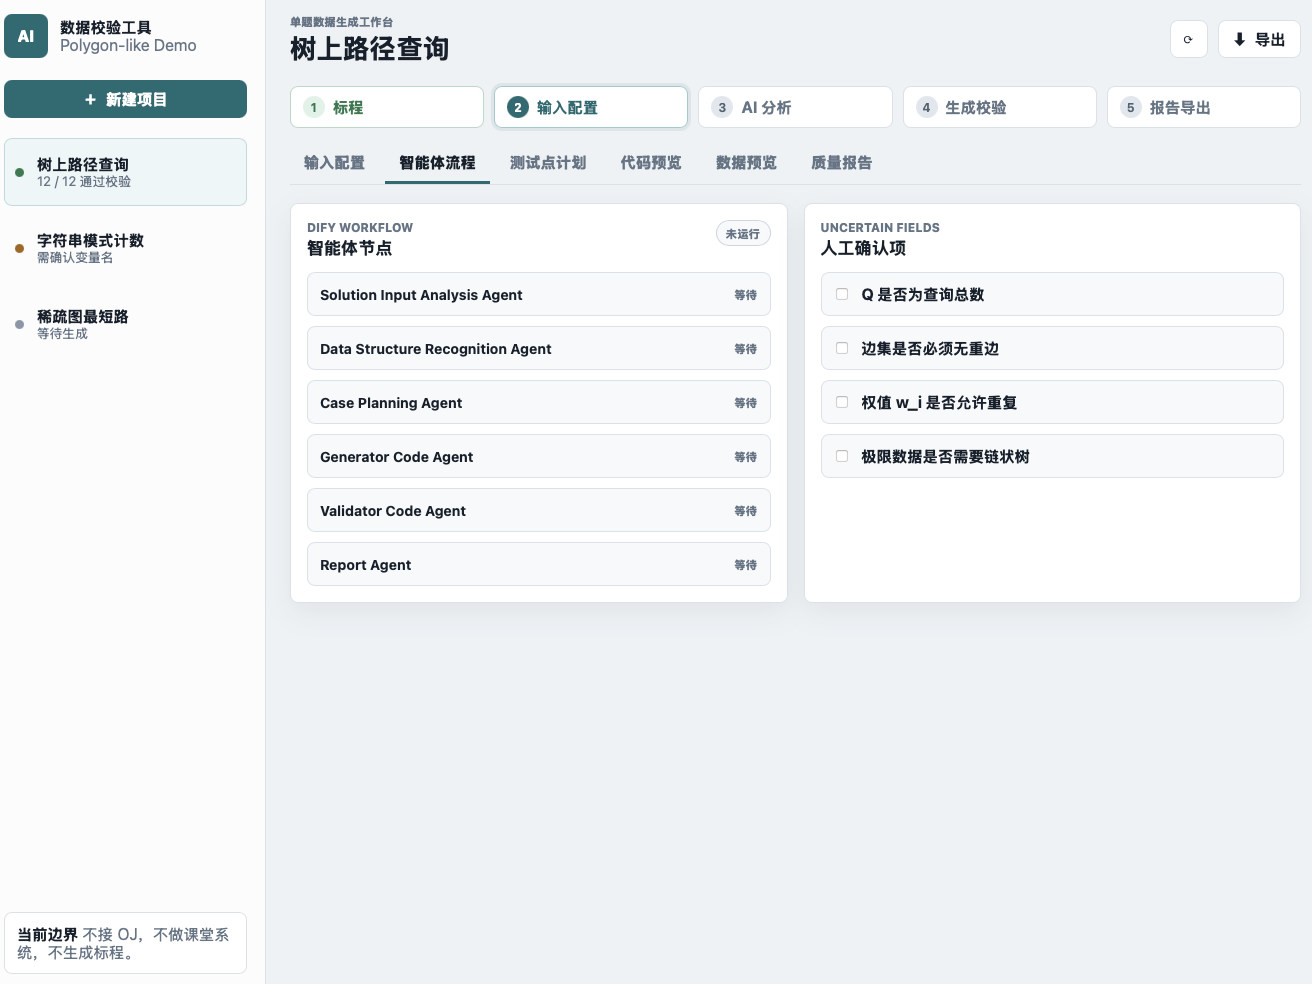
\includegraphics[width=0.8\textwidth]{智能体流程.png}}
  \caption{AI 处理与确认原型}
\end{figure}

\begin{figure}[H]
  \centering
  \colorbox{white}{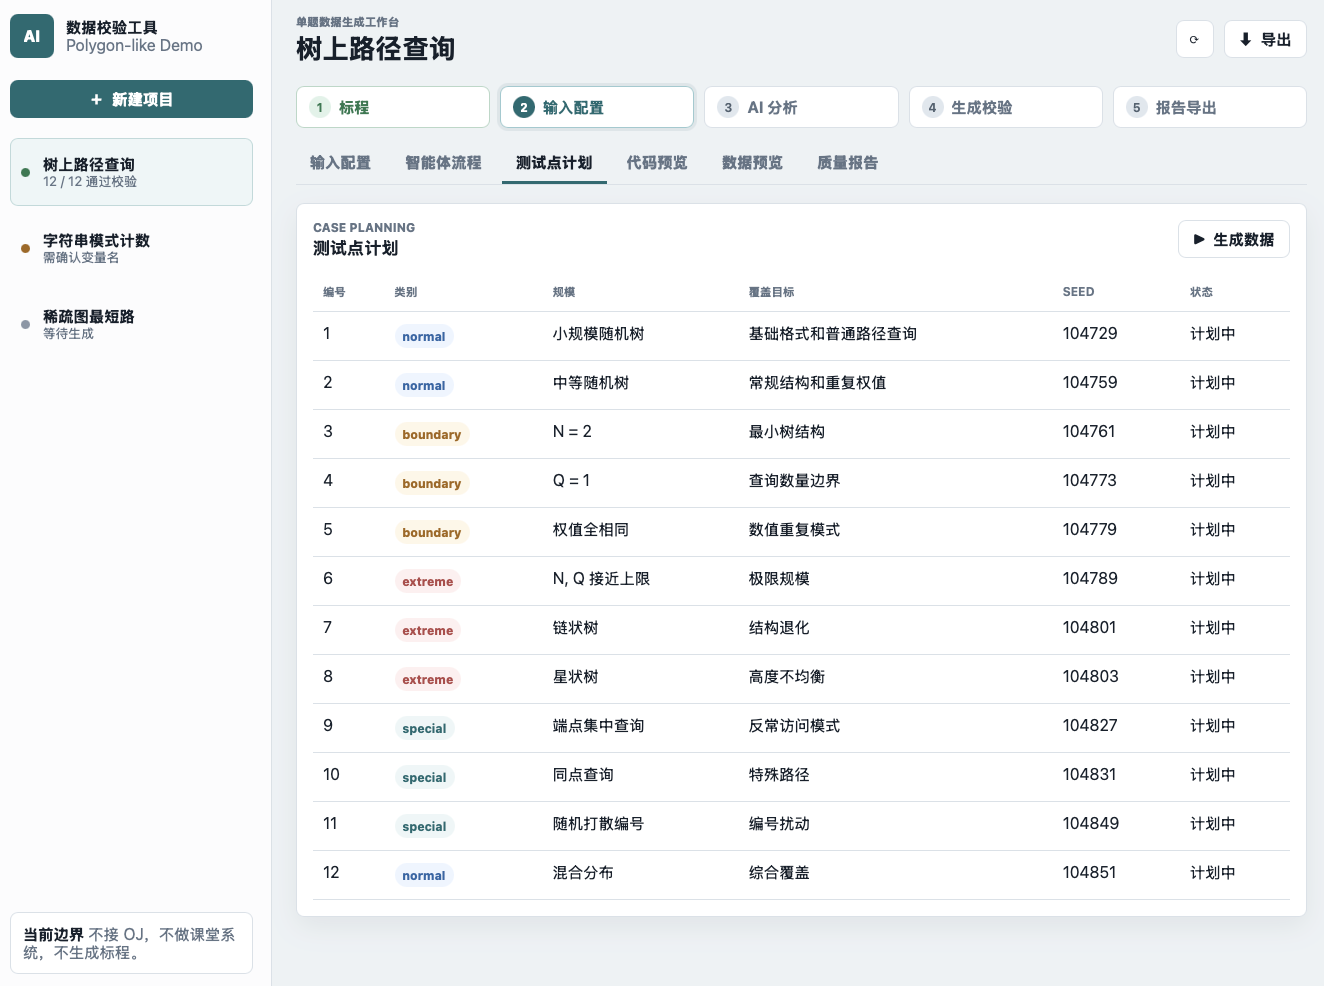
\includegraphics[width=0.8\textwidth]{测试点计划.png}}
  \caption{子任务规划原型}
\end{figure}

\begin{figure}[H]
  \centering
  \colorbox{white}{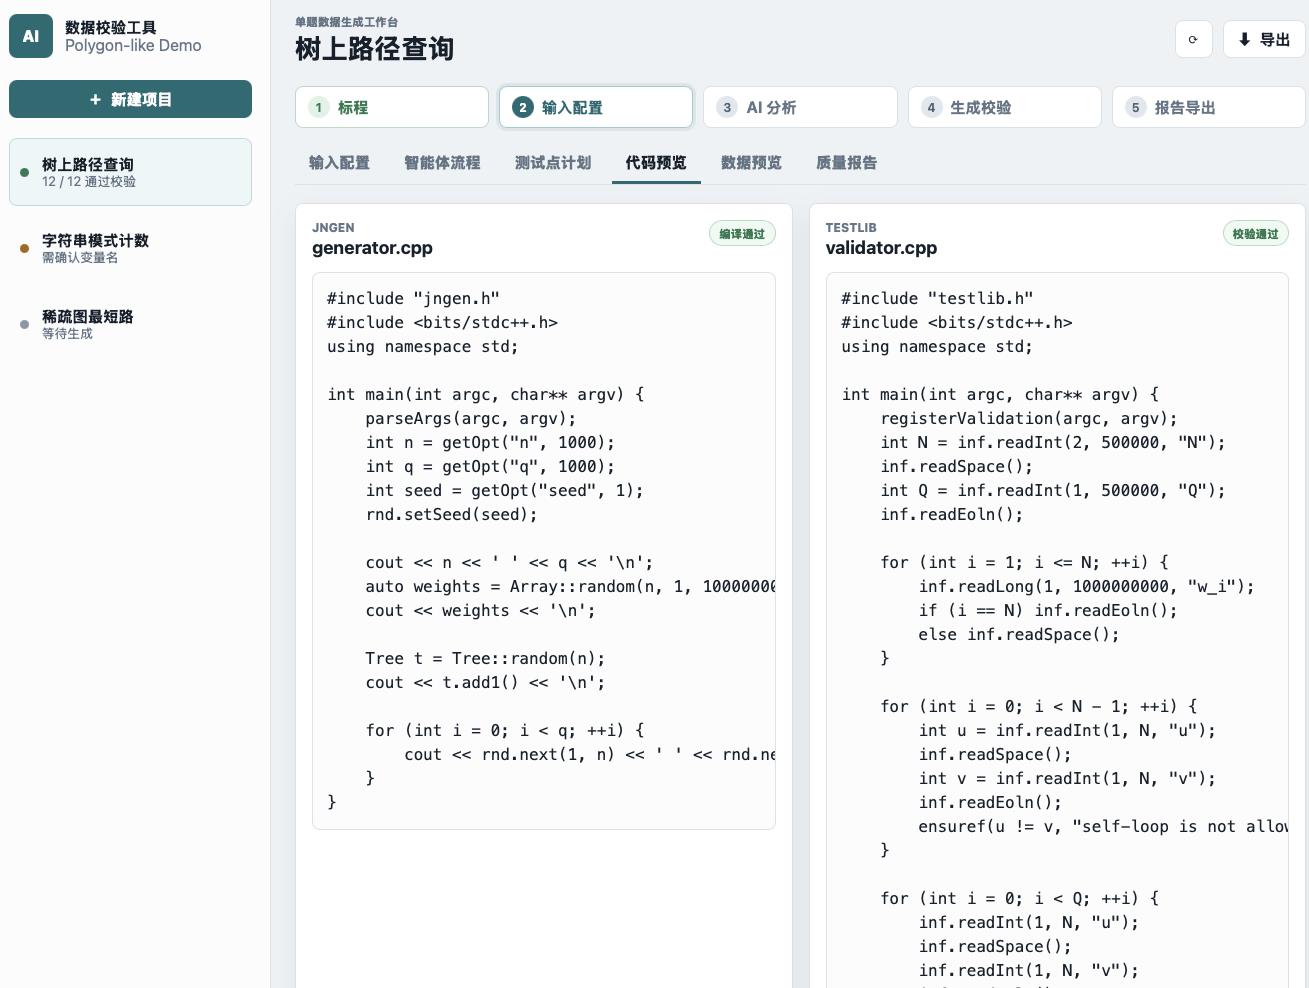
\includegraphics[width=0.8\textwidth]{代码预览.png}}
  \caption{生成器与校验器预览原型}
\end{figure}

\begin{figure}[H]
  \centering
  \colorbox{white}{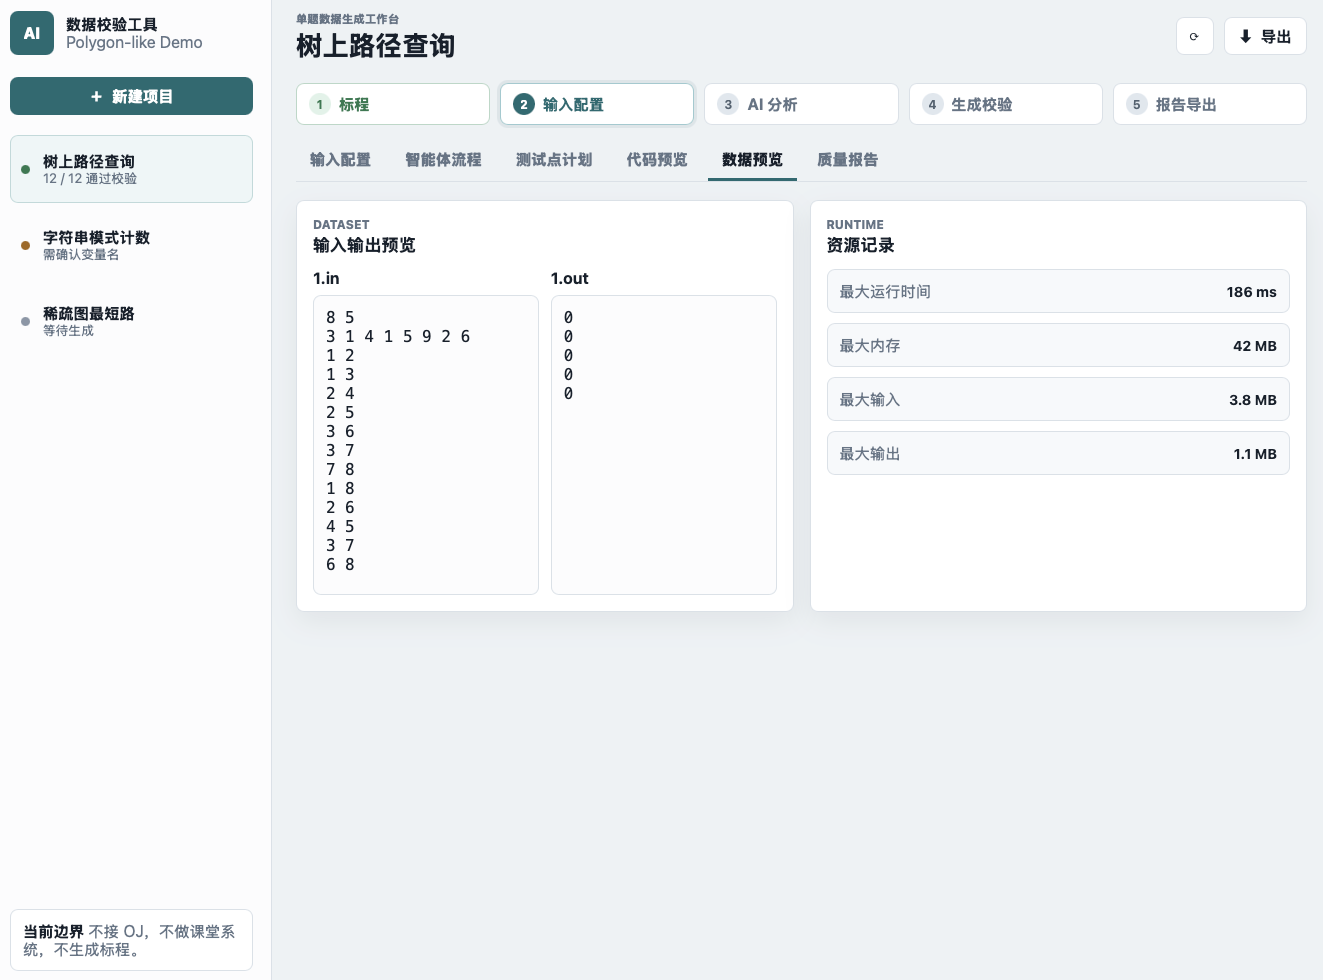
\includegraphics[width=0.8\textwidth]{数据预览.png}}
  \caption{数据预览原型}
\end{figure}

\end{document}
